\chapter{Complex Circuits with OpAmps}
\section{Ideal Half-Wave Rectifier}

\begin{figure}
	\centering
	\begin{subfigure}{0.44\textwidth}
		\centering
		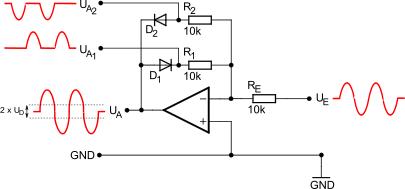
\includegraphics[width=\linewidth]{./img/schem-rectifier.pdf}
		\caption{Ideal Rectifier}
		\label{schem:rectifier}
	\end{subfigure}
	\begin{subfigure}{0.55\textwidth}
		\centering
		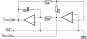
\includegraphics[width=\linewidth]{./img/schem-wavegen.pdf}
		\caption{Square and Triangle Wave Generator}
		\label{schem:wavegen}
	\end{subfigure}
	\caption{}
\end{figure}

\begin{figure}
	\centering
	\begin{subfigure}{0.4\textwidth}
		\centering
		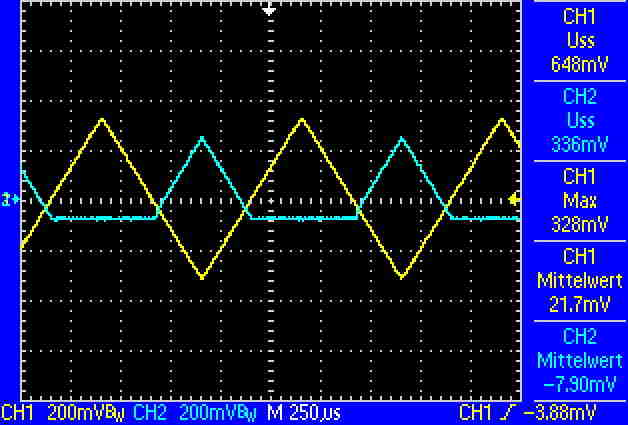
\includegraphics[width=.9\linewidth]{./img/ss-rect-pos}
		\caption{Positive Half Wave}
	\end{subfigure}
	\begin{subfigure}{0.4\textwidth}
		\centering
		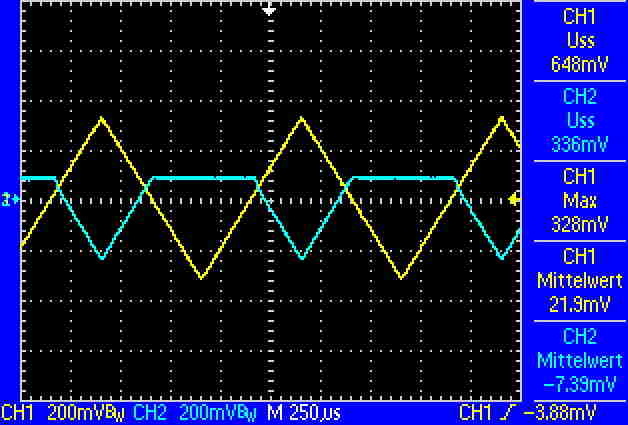
\includegraphics[width=.9\linewidth]{./img/ss-rect-neg}
		\caption{Negative Half Wave}
	\end{subfigure}
	\caption{Input (yellow) and Output (blue) of Ideal Rectifier}
	\label{ss:rect}
\end{figure}

\todo{image of output, slew rate}

A basic half-wave rectifier consists of a diode a resistor to provide a load to the diode.
All diodes carry an inherent voltage drop, so the signal level is lowered by \SI{0.2}{\volt} (Schottky diode) to \SI{0.7}{\volt} (silicon diode).
To combat this amplitude loss, an ideal rectifier is used.

An ideal rectifier (\autoref{schem:rectifier}) uses an operational amplifier with separate feedback paths for the positive and negative half wave.
Looking just at the output of the opamp, the two diodes in the feedback path are essentially anti-parallel, the rest forming an inverting ampifier with gain 1.
As the voltage drop due to the diodes in the feedback path is compensated by the feedback loop, the output of the opamp follows the input, with the amplitude increased by one diode drop.
This means that at zero crossings, in theory the output voltage is discontinuous, introducing high frequency components that may lead to undesired effects.

To now recover the rectified (or more specifically separated) positive and negative half waves, the circuit is tapped in the middle of each feedback line, where the output signal amplitude matches the input signal amplitude (this can be verified by looking at the two identical resistors connected to the inverting input: carrying the same current, they have an equal voltage across them with the inverting input being a virtual ground).

\section{Square and Triangle Wave Generator}

Operational amplifiers can also be operated with positive feedback.
As any perpetuation is amplified and fed back to the input in phase, the output voltage will not remain stable between the rails and is limited only by the rail voltage of the opamp.

By adding the output signal to the input signal, a bistable flip flop with different threshold voltages $U_{\text{thr, H} \rightarrow \text{L}} < U_{\text{thr, L} \rightarrow \text{H}}$, set by \comp{R_1} and \comp{R_2}, is created.
This circuit is called a non-inverting Schmitt trigger, and makes up the right portion of the circuit shown in \autoref{schem:wavegen}.

The left part of the circuit is an inverting integrator, it's output connected to the input of the Schmitt trigger.
As it receives either the positive or negative rail voltage, it acts as a ramp generator and ramps between the two threshold points of the Schmitt-trigger.
The resulting triangle wave is one output signal.
The other output signal is the square wave output of the Schmitt trigger, with a phase of \SI{90}{\degree} relative to the triangle signal.
The output signals are shown in \autoref{ss:wavegen}.

\begin{figure}
	\centering
	\begin{subfigure}{0.4\textwidth}
		\centering
		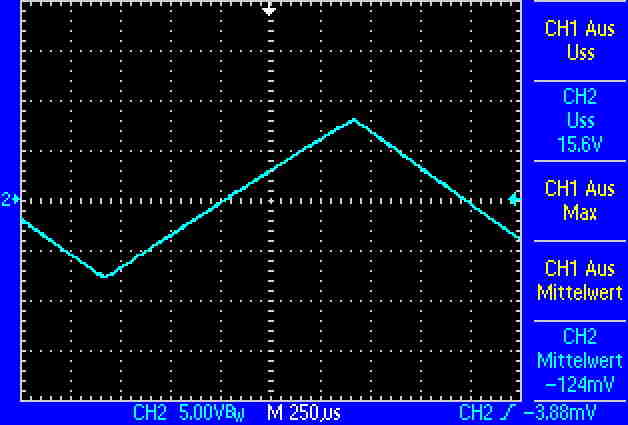
\includegraphics[width=.9\linewidth]{./img/ss-wavegen-triag}
		\caption{Triangle Wave Output Signal}
	\end{subfigure}
	\begin{subfigure}{0.4\textwidth}
		\centering
		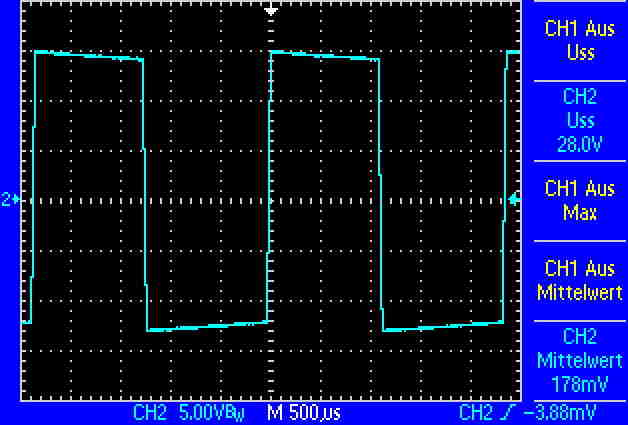
\includegraphics[width=.9\linewidth]{./img/ss-wavegen-squ}
		\caption{Square Wave Output Signal}
	\end{subfigure}
	\caption{Square and Triangle Wave Generator Waveforms}
	\label{ss:wavegen}
\end{figure}

\section{Programmable Differential Equation}

\begin{figure}
	\centering
	\begin{subfigure}{0.49\textwidth}
		\centering
		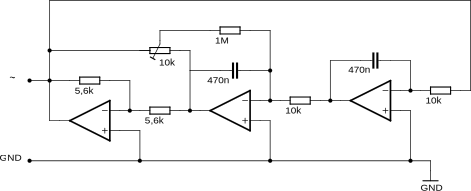
\includegraphics[width=\linewidth]{img/schem-dgl.pdf}
		\caption{Schematic}
		\label{schem:dgl}
	\end{subfigure}
	\begin{subfigure}{0.4\textwidth}
		\centering
		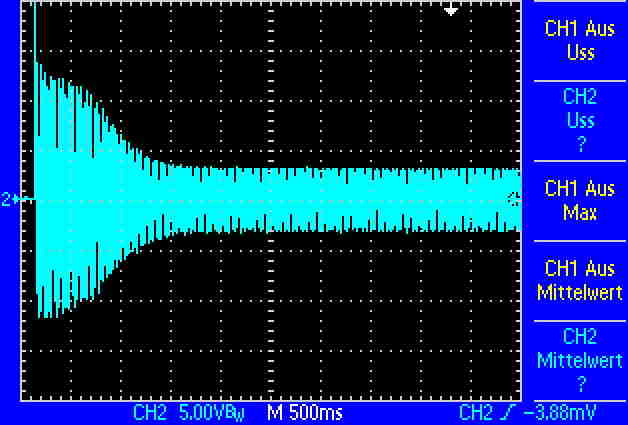
\includegraphics[width=.9\linewidth]{./img/ss-dgl.jpg}
		\caption{Output Waveform}
		\label{ss:dgl}
	\end{subfigure}
	\caption{Programmable Differential Equation}
\end{figure}

Integrators can be used to 'numerically' solve ordinary differential equations.
As an example, the ordinary second order linear differential equation \[\ddot{x} = - 2 \gamma \dot{x} - \omega^2 x\] is implemented with opamps as shown in \autoref{schem:dgl}.

Two inverting integrators form the core of the circuit, the leftmost opamp inverts $x$ to obtain the $-\omega^2 x$ oscillation term.
The dampening term $-2\gamma\dot{x}$ is implemented by feeding a voltage between $-x$ and $x$, selected by the potentiometer, back into $\dot{x}$.

The possibility for oscillations can also be verified by analyzing the loop stability of the circuit.
The integrators each introduce a phase shift of \SI{90}{\degree} and together with the leftmost inverting amplifier they add up to positive feedback with a phase of \SI{360}{\degree}, which, among with a total loop gain grater than unity, is the condition for oscillations to occur.\todo{please fact check, hodenkobold}

To start an oscillation, a voltage has to be applied at an arbitrary high-impedance point of the circuit.
\autoref{ss:dgl} show the output waveform of the circuit after being excited by applying the rail voltage to the inverting input of the leftmost amplifier.
The oscillation does decay over time, but it does not completely stop.
This is likely an effect of imperfections of the used components.
